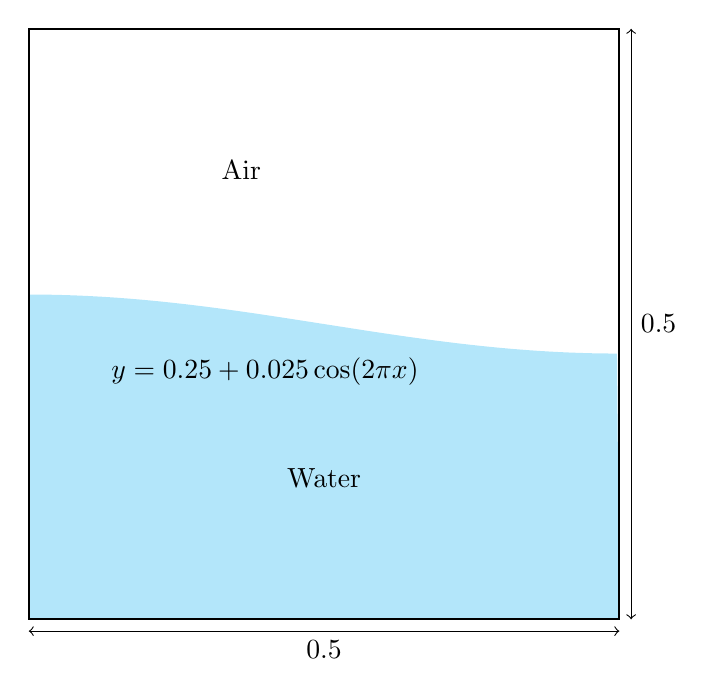
\begin{tikzpicture}[scale=15]


% Water region (blue fill, below interface)
\fill[cyan!30, domain=0:0.5, samples=200]
(0,0)
-- plot (\x, {0.25 + 0.025*cos(360*\x)})
-- (0.5,0)
-- cycle;

% Phase labels
\node at (0.18,0.38) {Air};
\node at (0.25,0.12) {Water};

% Gravity vector
% \draw[->, thick] (0.3,0.35) -- (0.3,0.25)
% node[midway, right] {$\boldsymbol{g}=(0,-2\pi)^{\mathrm{T}}$};

% ---- Dimension annotations ----
% Horizontal length 0.5
\draw[<->] (0,-0.01) -- (0.5,-0.01)
node[midway, below] {$0.5$};

% Vertical length 0.5
\draw[<->] (0.51,0) -- (0.51,0.5)
node[midway, right] {$0.5$};

% ---- Interface annotation ----
\node at (0.2,0.21)
{$y=0.25+0.025\cos(2\pi x)$};

% Domain boundary
\draw[thick] (0,0) rectangle (0.5,0.5);


\end{tikzpicture}
